\documentclass[a4paper,10pt,twocolumn]{article}
\usepackage{cite}
\usepackage{listings}
\usepackage[T1]{fontenc}
\usepackage{amsmath}
\usepackage{amssymb}
\usepackage{graphicx}
\usepackage[]{circuitikz}
\setlength{\oddsidemargin}{0in}
\setlength{\topmargin}{-.8in}
\setlength{\textheight}{9.7in} \setlength{\textwidth}{6.5in}
\usepackage{color,hyperref}
\definecolor{darkblue}{rgb}{0.0,0.0,0.3}
\hypersetup{colorlinks,breaklinks,
            linkcolor=darkblue,urlcolor=darkblue,
            anchorcolor=darkblue,citecolor=darkblue}
\providecommand*\url[1]{\href{#1}{#1}}
\renewcommand*\url[1]{\href{#1}{\texttt{#1}}}

\newcommand{\bm}[1]{\boldsymbol{#1}}
\newcommand{\bh}[1]{\boldsymbol{\hat{#1}}}
\newcommand{\bt}[1]{\boldsymbol{\tilde{#1}}}
\newcommand{\bbar}[1]{\boldsymbol{\bar{#1}}}
\newcommand{\mbf}[1]{\ensuremath{\mathbf{#1}}}
\newcommand{\ode}[2]{\ensuremath{\frac{\mathrm{d} #1}{\mathrm{d} #2}}}
\newcommand{\odet}[2]{\ensuremath{\tfrac{\mathrm{d} #1}{\mathrm{d} #2}}}
\newcommand{\oden}[3]{\ensuremath{\frac{\mathrm{d}^#3 #1}{\mathrm{d} #2^#3}}}
\newcommand{\pde}[2]{\ensuremath{\frac{\partial #1}{\partial #2}}}
\newcommand{\pdet}[2]{\ensuremath{\tfrac{\partial #1}{\partial #2}}}
\newcommand{\pden}[3]{\ensuremath{\frac{\partial^{#3} #1}{\partial
      #2^{#3}}}}
\newcommand{\sub}[1]{\ensuremath{_{\rm{#1}}}}
\newcommand{\arriba}[1]{\ensuremath{^{\rm{#1}}}}
%
\newcommand{\N}{\ensuremath{\mathbb{N}}}
\newcommand{\R}{\ensuremath{\mathbb{R}}}
\newcommand{\C}{\ensuremath{\mathbb{C}}}
\newcommand{\ee}[1]{\ensuremath{\mathrm{e}^{#1}}}
\newcommand{\hdos}{\ensuremath{\mathrm{H}_2}}
\newcommand{\COdos}{\ensuremath{\mathrm{CO}_2}}
\newcommand{\ATP}{\ensuremath{\mathrm{ATP}}}

\newcommand{\dt}{\ensuremath{\mathrm{d}t}}
\newcommand{\dtau}{\ensuremath{\mathrm{d}\tau}}
\newcommand{\DV}{\ensuremath{\Delta V}}

\DeclareMathOperator{\Li}{\mathcal {L}^{-1}}
\DeclareMathOperator{\Lin}{\mathcal {L}^{-1}}
\DeclareMathOperator{\sinc}{\text{sinc}}
\DeclareMathOperator{\sign}{\mathrm{sign}}
\DeclareMathOperator{\diag}{\mathrm{diag}}


\newtheorem{remark}{Remark}
\newtheorem{prob}{Problem}

\usepackage[utf8x]{inputenc}
%%

\title{Support Vector Machines\\ Optimization \\ DMKM}
\author{Carlos López Roa\\ \href{mailto:me@mr3m.me}{me@mr3m.me} }
\date{\today}
\pdfinfo{%
  /Title    ()
  /Author   (CLR)
  /Creator  ()
  /Producer ()
  /Subject  ()
  /Keywords ()
}
\begin{document}
\maketitle
\lstset{
language={matlab},
basicstyle=\tiny,
numbers=left,
numberstyle=\tiny,
numbersep=5pt, 
showspaces=false,
showstringspaces=false,
showtabs=False,
frame=false,
%tabsize=.5,
keywordstyle=\bfseries\color{green!40!black},          % keyword style
 commentstyle=\itshape\color{purple!40!black},       % comment style
 identifierstyle=\color{blue},
  stringstyle=\color{orange},
basicstyle=\ttfamily,
captionpos=b}
\lstdefinestyle{matlab}{
language={matlab},
basicstyle=\tiny,
numbers=right,
numberstyle=\tiny,
numbersep=5pt, 
showspaces=false,
showstringspaces=false,
showtabs=False,
frame=single,
tabsize=.5,
keywordstyle=\bfseries\color{green!40!black},          % keyword style
 commentstyle=\itshape\color{purple!40!black},       % comment style
 identifierstyle=\color{blue},
  stringstyle=\color{orange},
basicstyle=\ttfamily,
captionpos=b,
title=\lstname
}
%%% Content
\section*{Abstract}
We used a Support Vector Machine (SVM) to train a binary classifier. 
\section*{Introduction}
Given a $m$ vectors in $\mathbb{R}^n$ represented in the matrix $A \in \R^{m\times n}$ labeled by the binary vector $\hat{y}$ with $\hat{y}_i \in \{-1,1\}$, we can construct the \emph{linear kernel support vector machine} with the quadratic optimization problem: 
\begin{prob}\label{prob1}
\begin{equation}
\begin{aligned}
\min_{\omega,\gamma,y} &\hspace{0.5cm} \nu e^T y +\frac{1}{2}\omega^T\omega\\
s.t. &\hspace{0.5cm} D\times(A\omega - e \gamma)+y\geq e\\
&\hspace{0.5cm} y \geq 0.
\end{aligned}
\end{equation}
With $\omega \in \mathbb{R}^n, \, \gamma \in \R, \, y \in \R^m, \, e=\mathbf{1} \in\mathbb{R}^m, \nu >0$ and $D=\diag(\hat{y})$.
\end{prob}
Recall $||x||_2^2=\langle x,x\rangle=x^Tx$. The solution of problem \ref{prob1}  defines a hyperplane 
\begin{equation}
\begin{aligned}
x^T\omega = \gamma, 
\end{aligned}
\end{equation}
which separate the points represented in matrix $A$ into two semispaces.

Thus we are to evaluate the error of the classifier using the formula 
\begin{equation}
\begin{aligned}
\epsilon&=\frac{1}{2m}\sum|\sign(A\omega-\gamma)-\hat{y}|
\end{aligned}
\end{equation}

\section*{Implementation}
We chose to implement the \texttt{CVX} solver in \texttt{Matlab 2011a}  \texttt{7.12.0.635}.

First we generated the data using the provided binary of sizes $10^1,10^2,10^3,10^4$, with seed \texttt{26071991}.

Then we parsed the output into \texttt{txt} files using the supplied code in python, removing the special cases marked with \texttt{*} as follows

\begin{lstlisting}[language=python]
i=1
f1 = open('x10.txt','w')
f2 = open('y10.txt','w')
with open('10.dat','r') as rf:
    reader = csv.reader(rf,delimiter=' ')
    for row in reader:
        if "*" not in row[6]:
            f1.write(row[0]+' '+row[1]+' '
		+row[2]+' '+row[3]+'\n')
            f2.write(row[6]+'\n')
        i += 1
f1.close() 
f2.close()
\end{lstlisting}

The following is to call the solver in \texttt{Matlab}

\begin{lstlisting}[language=matlab]
err = []; temp =[]; i=3;
At=importdata('x100000.txt');
ytt=importdata('y100000.txt');
sizes=[10,100,1000,10000,100000];
A=At(1:sizes(i),1:4);
yt=ytt(1:sizes(i));
[m n]=size(A); nu=2^(7-10); e=ones(m,1);
cvx_begin quiet
    variables w(n) gam y(m)
    minimize (nu*e'*y+(0.5)*w'*w)
      subject to
      diag(yt)*(A*w-e*gam) + y >= e 
      y >= 0
cvx_end
\end{lstlisting}

Where we used the best $\nu$ we could find discussed in the results.
\section*{Results}
To choose the best $\nu$ in order to minimize the error trying not to overfit, we explored the parameter iterating on the range $\{2^{i}\}_{i=-9}^{10}$ exhibiting the result shown in figure \ref{fig1}. We chose the minimum $\nu$ in the \emph{sweet} zone, that is $\nu=2^{-3}$

\begin{figure}[!ht]
\begin{center}
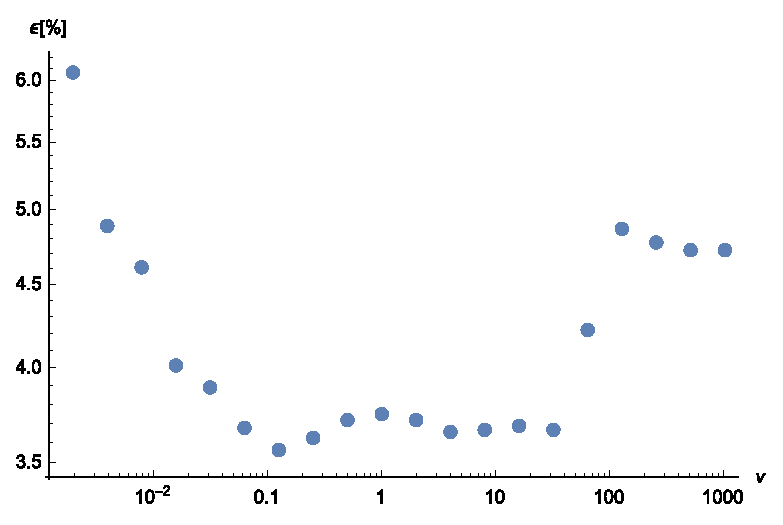
\includegraphics[width=7cm]{ex1.eps}
\caption{\footnotesize{Behaviour of the error as a function of the parameter $\nu$ we observe a \emph{sweet} zone in which the error stays low, before going up again.}\label{fig1}}
\end{center}
\end{figure}

Using this parameter we chose to train a $10^3$ sample size and test in a $10^4$ sample size, that is training with just $10\%$ of the sample. 

The results as follows:
$$
\begin{tabular}{ |l |c | c | }
\hline
$m$ & $\epsilon$[\%]   \\
\hline			
  $10^3$ & 4.8  \\
  $10^4$ & 5.0  \\
  \hline  
\end{tabular}
$$
That is, the sample set exhibited $95.2\%$ accuracy and the test set $95\%$ using only 10\% of the set to train. 

\section*{Conclusions}
\begin{enumerate}
\item We implemented a linear kernel suppor vector machine to classify a binary labeled set in $\R^4$
\item We explored the normalization parameter of the model to minimize the error still avoiding overfitting.
\item We trained the model using only $10\%$ of the test set and got accuracy of $95\%$ 
\end{enumerate}

\end{document}